% !TEX program = lualatex
% !TeX TS-program = lualatex
% Unofficial University of Cambridge Poster Template
% https://github.com/andiac/gemini-cam
% a fork of https://github.com/anishathalye/gemini
% also refer to https://github.com/k4rtik/uchicago-poster

\documentclass[final]{beamer}

% ====================
% Packages
% ====================

\usepackage[T1]{fontenc}
\usepackage{lmodern}
\usepackage[orientation=portrait,size=a0,scale=1.15]{beamerposter}
\usetheme{gemini}
\usecolortheme{nott}

% Custom color scheme
\usepackage{xcolor}
\definecolor{darkgray}{HTML}{334443}        % Dark gray for headers/footers
\definecolor{tealblue}{HTML}{34656D}        % Teal blue for block titles
\definecolor{creamwhite}{HTML}{FAF8F1}      % Cream white for backgrounds
\definecolor{lightyellow}{HTML}{FAEAB1}     % Light yellow for alert blocks

% Apply custom colors
\setbeamercolor{headline}{bg=darkgray}
\setbeamercolor{footline}{bg=darkgray}
\setbeamercolor{block title}{bg=tealblue,fg=white}
\setbeamercolor{block body}{bg=creamwhite,fg=black}
\setbeamercolor{block title alerted}{bg=lightyellow,fg=darkgray}
\setbeamercolor{block body alerted}{bg=creamwhite,fg=black}

% Remove underline from block titles
\setbeamertemplate{block begin}{
  \par\vskip\medskipamount%
  \begin{beamercolorbox}[colsep*=.75ex]{block title}
    \usebeamerfont*{block title}\insertblocktitle%
  \end{beamercolorbox}%
  {\parskip0pt\par}%
  \ifbeamercolorempty[bg]{block title}
  {}
  {\ifbeamercolorempty[bg]{block body}{}{\nointerlineskip\vskip-0.5pt}}%
  \usebeamerfont{block body}%
  \begin{beamercolorbox}[colsep*=.75ex,vmode]{block body}%
    \ifbeamercolorempty[bg]{block body}{\vskip-.25ex}{\vskip-.75ex}\vbox{}%
}
\setbeamertemplate{block end}{
  \end{beamercolorbox}\vskip\smallskipamount
}

% Remove underline from alert blocks
\setbeamertemplate{block alerted begin}{
  \par\vskip\medskipamount%
  \begin{beamercolorbox}[colsep*=.75ex]{block title alerted}
    \usebeamerfont*{block title alerted}\insertblocktitle%
  \end{beamercolorbox}%
  {\parskip0pt\par}%
  \ifbeamercolorempty[bg]{block title alerted}
  {}
  {\ifbeamercolorempty[bg]{block body alerted}{}{\nointerlineskip\vskip-0.5pt}}%
  \usebeamerfont{block body alerted}%
  \begin{beamercolorbox}[colsep*=.75ex,vmode]{block body alerted}%
    \ifbeamercolorempty[bg]{block body alerted}{\vskip-.25ex}{\vskip-.75ex}\vbox{}%
}
\setbeamertemplate{block alerted end}{
  \end{beamercolorbox}\vskip\smallskipamount
}

\usepackage{graphicx}
\usepackage{booktabs}
\usepackage{tikz}
\usepackage{pgfplots}
\pgfplotsset{compat=1.14}
\usepackage{anyfontsize}
\usepackage{caption}
\captionsetup[figure]{labelformat=empty}


% ====================
% Lengths
% ====================

% If you have N columns, choose \sepwidth and \colwidth such that
% (N+1)*\sepwidth + N*\colwidth = \paperwidth
\newlength{\sepwidth}
\newlength{\colwidth}
\setlength{\sepwidth}{0.025\paperwidth}
\setlength{\colwidth}{0.45\paperwidth}

\newcommand{\separatorcolumn}
{\begin{column}{\sepwidth}\end{column}}

% ====================
% Title
% ====================

\title{Instant Particle Size Distribution Measurement Using CNNs Trained on Synthetic Data}

\author{Yasser El Jarida, Youssef Iraqi, Loubna Mekouar}

\institute[shortinst]{College of Computing, Mohammed VI Polytechnic University \samelineand}

% ====================
% Footer (optional)
% ====================

\footercontent{
  \href{https://cc.um6p.ma/home}{UM6P COLLEGE OF COMPUTING} \hfill
  \hfill
  Published at CVPR 2025 SynData4CV Workshop, Nashville, USA \hspace{2em} \textbf{Poster \#235}
}
% (can be left out to remove footer)


% ====================
% Logo (optional)
% ====================

% use this to include logos on the left and/or right side of the header:
\logoright{\raisebox{1.5cm}{
\includegraphics[scale=1.4]{logo_um6p_cc_white.png}}}
\logoleft{\raisebox{2.25cm}{
\includegraphics[scale=2.5]{logoum6p_white.png}}}

% ====================
% Body
% ====================

\begin{document}

% Add poster number under logo
\addtobeamertemplate{headline}{}
{
    \begin{tikzpicture}[remember picture,overlay]
      \node [anchor=north west, inner sep=0cm] at ([xshift=3cm,yshift=-12.5cm]current page.north west)
      {\fontsize{48}{60}\selectfont\textcolor{white}{\textbf{Poster~\#235}}};
    \end{tikzpicture}
}

\begin{frame}[t]
\begin{columns}[t]
\separatorcolumn

\begin{column}{\colwidth}

  \begin{alertblock}{Motivation}

    \textbf{Context:} Particle size distribution is a key characteristic that influences how phosphate behaves in various contexts, including phosphate rock processing, soil chemistry, and industrial applications. The distribution, or the proportion of particles in a given size range, directly affects important properties like surface area, reactivity, and physical handling.

    \textbf{Problem:} Traditional methods are costly (data collection, labeling, etc.) and slow. Creating a high-quality, diverse dataset with reliable labels is time-consuming, error-prone, and difficult to scale. It is a real pain to make such a dataset manually.

    \textbf{Our Solution:} We leverage realistically rendered synthetic data generated with Blender to provide automatic, perfectly labeled supervision for key PSD metrics (d10, d50, d90), enabling robust CNN training without manual annotation. We open-source our data generation pipeline and training framework to accelerate research in automated PSD estimation.

  \end{alertblock}

  \begin{figure}
      \centering
      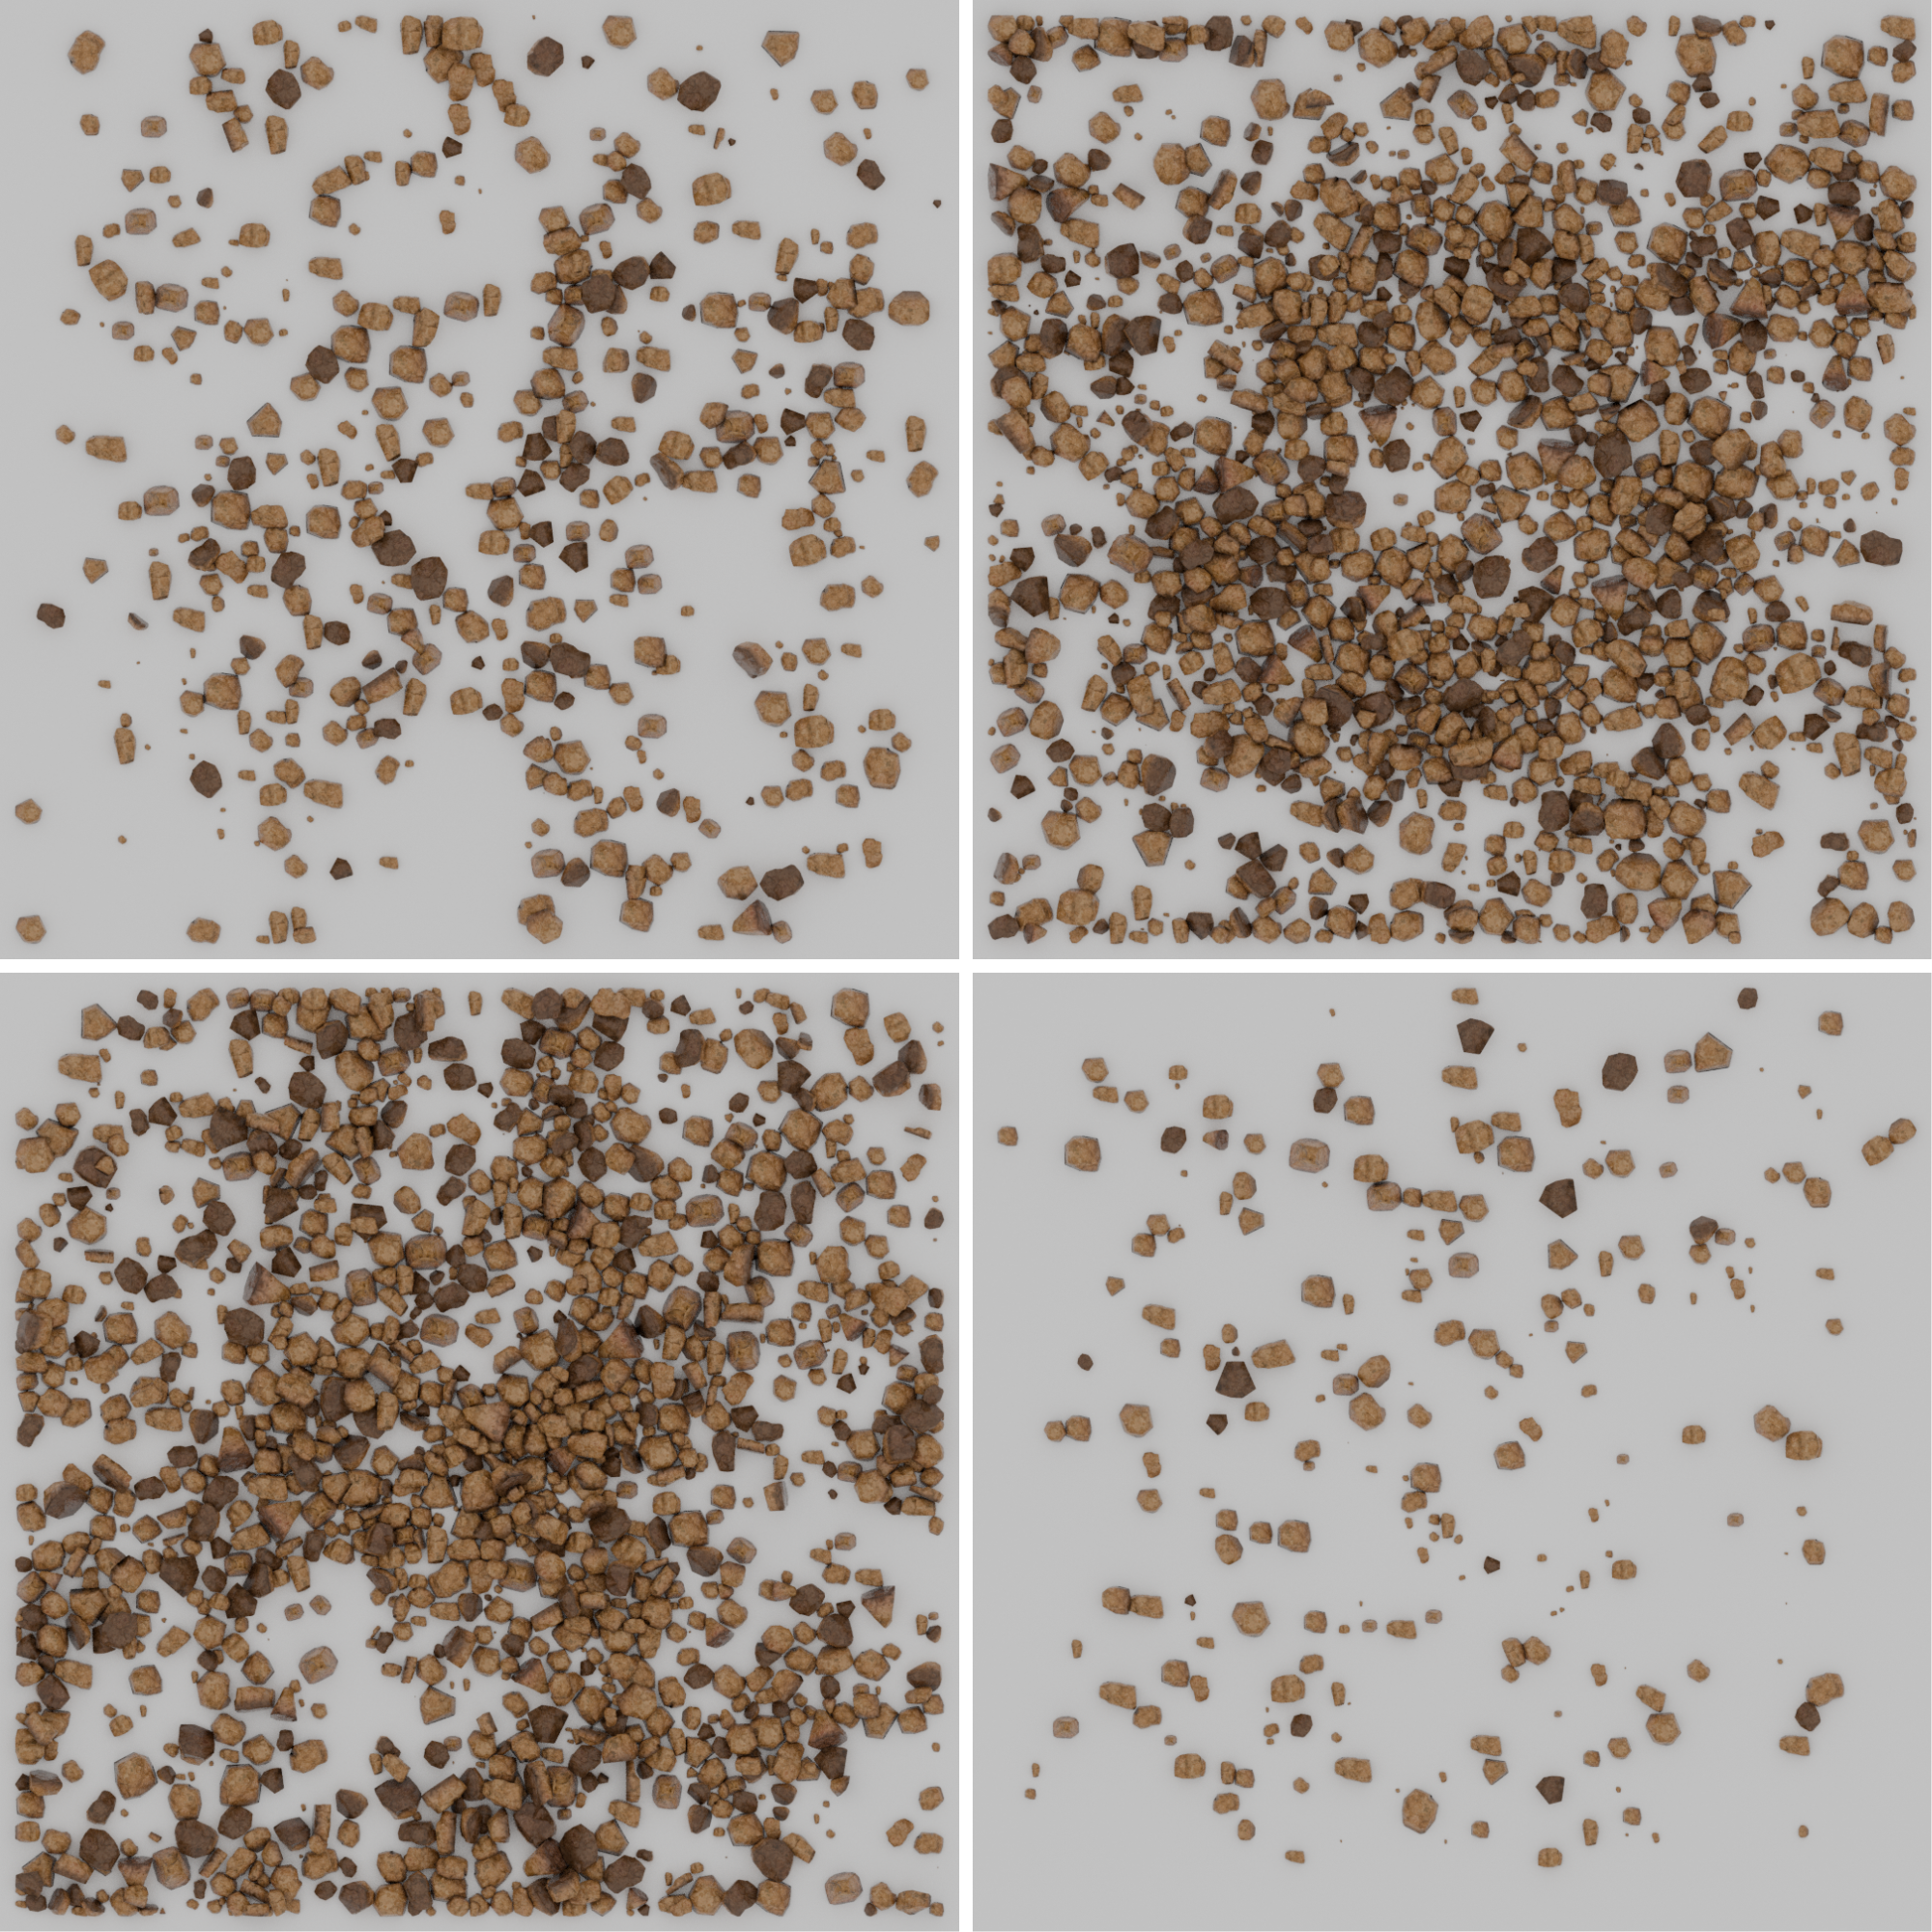
\includegraphics[width=1\linewidth]{Synthetic_Data_for_Computer_Vision___CVPR_2025/figures/samples_square.png}
      \caption{Realistic synthetic particle images with controlled size distributions and perfect labels.}
      \label{fig:samples}
  \end{figure}

  \begin{block}{Methodology}

  \heading{Synthetic Data Generation Pipeline}
  
  We developed a fully automated Blender-based pipeline with two main components:
  
  \begin{itemize}
    \item \textbf{Metadata Generation:} Randomly samples particle count (700-1000), sizes from truncated normal distribution $\mathcal{N}_T(\mu, \sigma^2; a, b)$ where $\mu \in [6,12]$mm, $\sigma \in [6,8]$mm, truncated to $[a, b] = [0.1, 20]$mm, and positions. Outputs structured JSON with exact PSD ground truth (d10, d50, d90).
    \item \textbf{Scene Construction \& Rendering:} Loads 3D particle meshes with realistic textures (base color, metallic, roughness, normal maps), runs rigid-body physics simulation, renders with Cycles engine (GPU-accelerated). ~4,500 images rendered on HPC A100 GPUs.
  \end{itemize}

  \begin{figure}
      \centering
      \begin{minipage}[b]{0.32\textwidth}
        \centering
        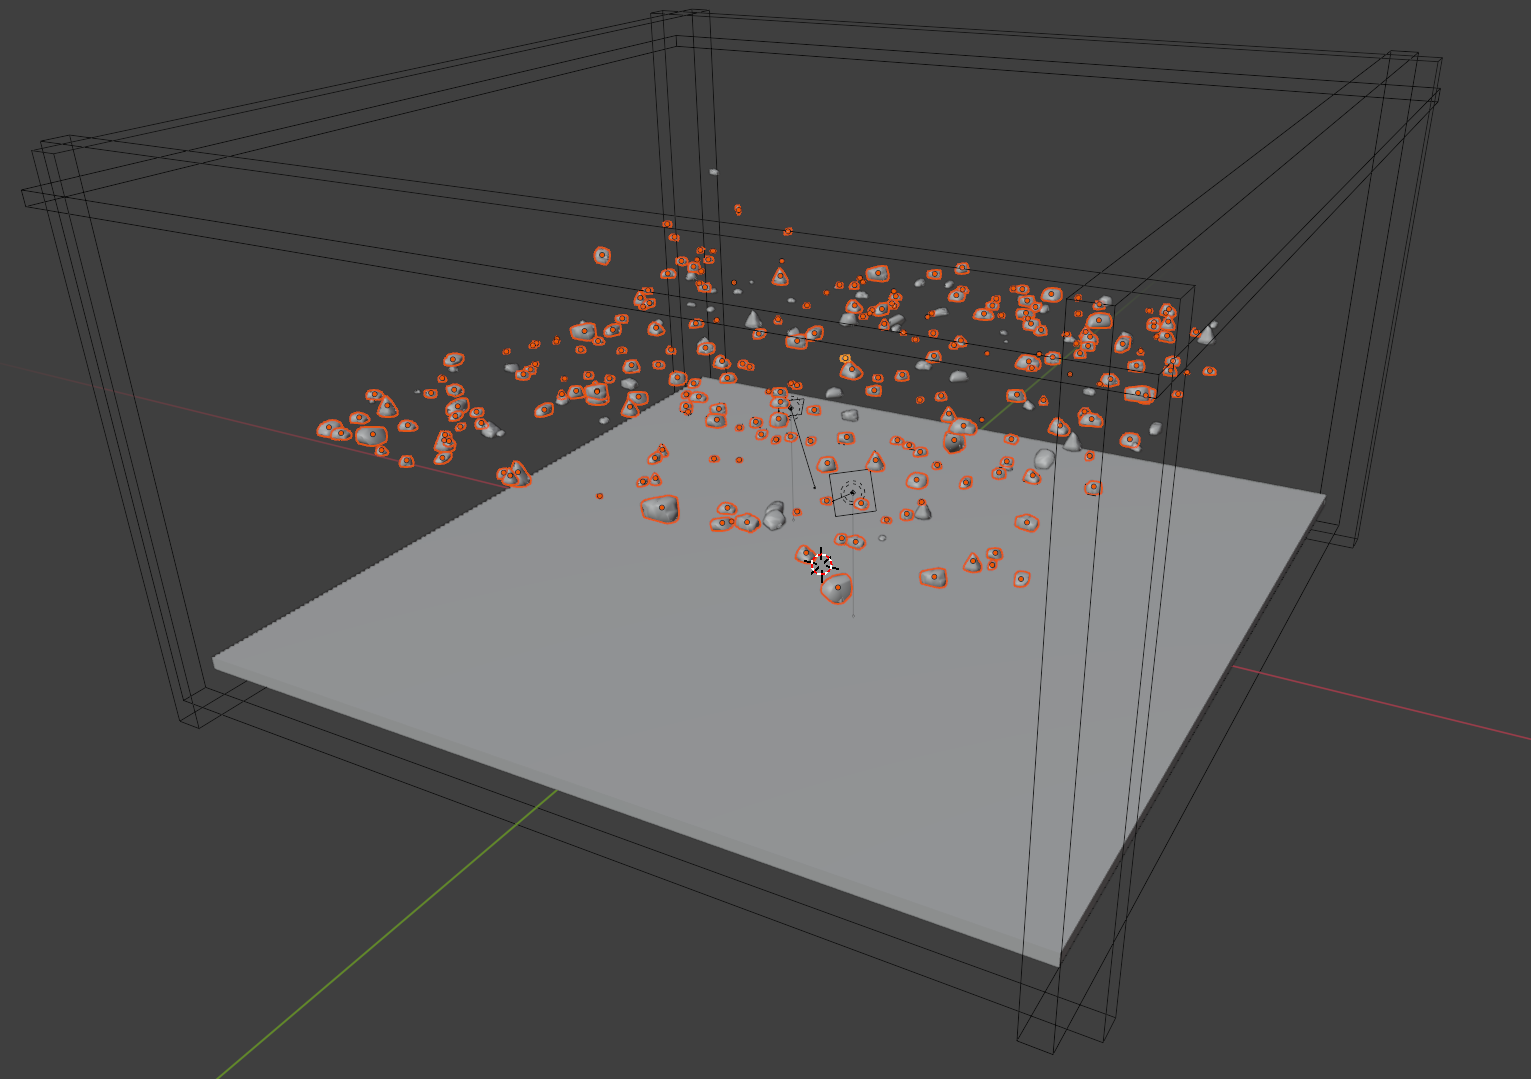
\includegraphics[width=\linewidth]{Synthetic_Data_for_Computer_Vision___CVPR_2025/figures/blender_interface.png}
        \caption{Blender setup}
      \end{minipage}\hfill
      \begin{minipage}[b]{0.32\textwidth}
        \centering
        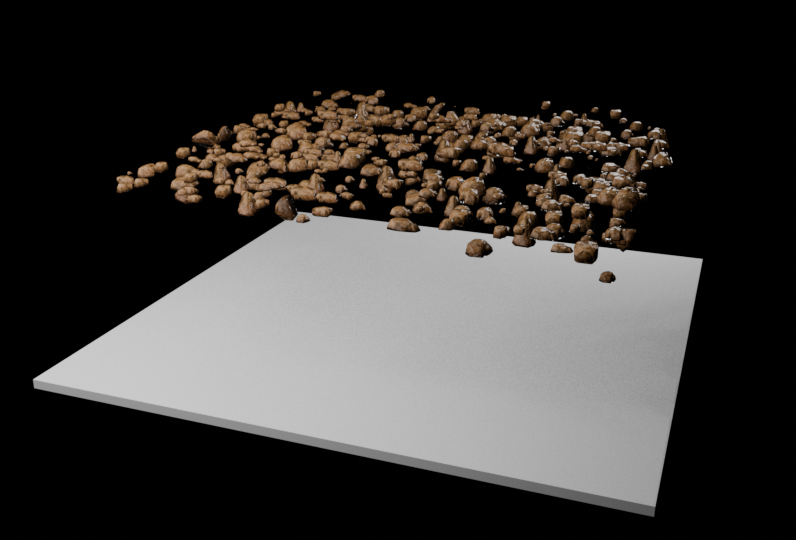
\includegraphics[width=\linewidth]{Synthetic_Data_for_Computer_Vision___CVPR_2025/figures/blender_rendered.png}
        \caption{Rendered scene}
      \end{minipage}\hfill
      \begin{minipage}[b]{0.32\textwidth}
        \centering
        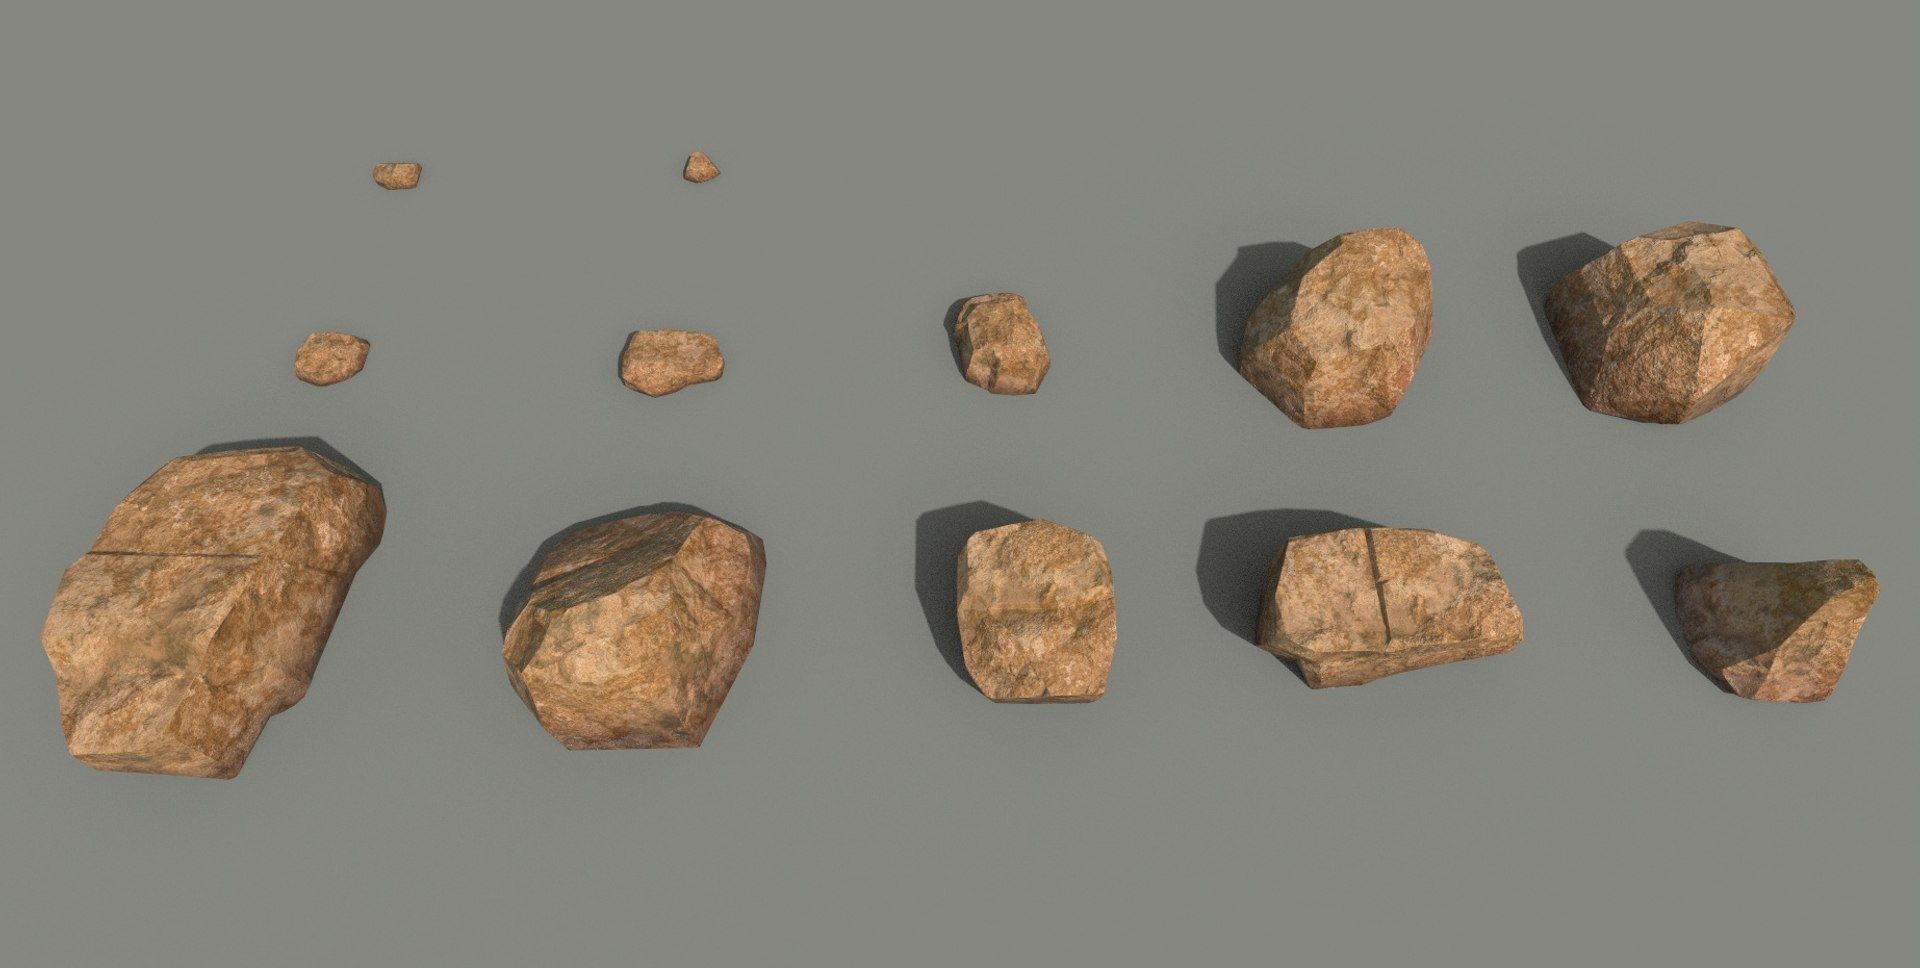
\includegraphics[width=\linewidth]{Synthetic_Data_for_Computer_Vision___CVPR_2025/figures/rock_models.png}
        \caption{Particle models}
      \end{minipage}
  \end{figure}
  \vspace{-1em}
  \heading{CNN Training}
  
  Three architectures evaluated: ResNet-50, InceptionV3, EfficientNet-B0 (all ImageNet-pretrained).
  \begin{itemize}
    \item Fine-tuned for regression (d10, d50, d90) with MSE loss, Adam optimizer (lr=$10^{-4}$)
    \item Data augmentation: rotations (0°, 90°, 180°, 270°), horizontal flips
    \item Trained 50 epochs on HPC A100 GPUs (~3 hours per model)
  \end{itemize}

  \end{block}

\end{column}

\separatorcolumn

\begin{column}{\colwidth}

  \begin{block}{Experimental Results}

  \heading{Prediction Accuracy}
  
  All three models achieve high accuracy on synthetic test data. ResNet-50 shows marginally better performance (R²=0.9987, MAE=0.077mm), but differences are minor (<0.1mm) across d10, d50, d90 predictions.

  \begin{figure}[h]
        \centering
        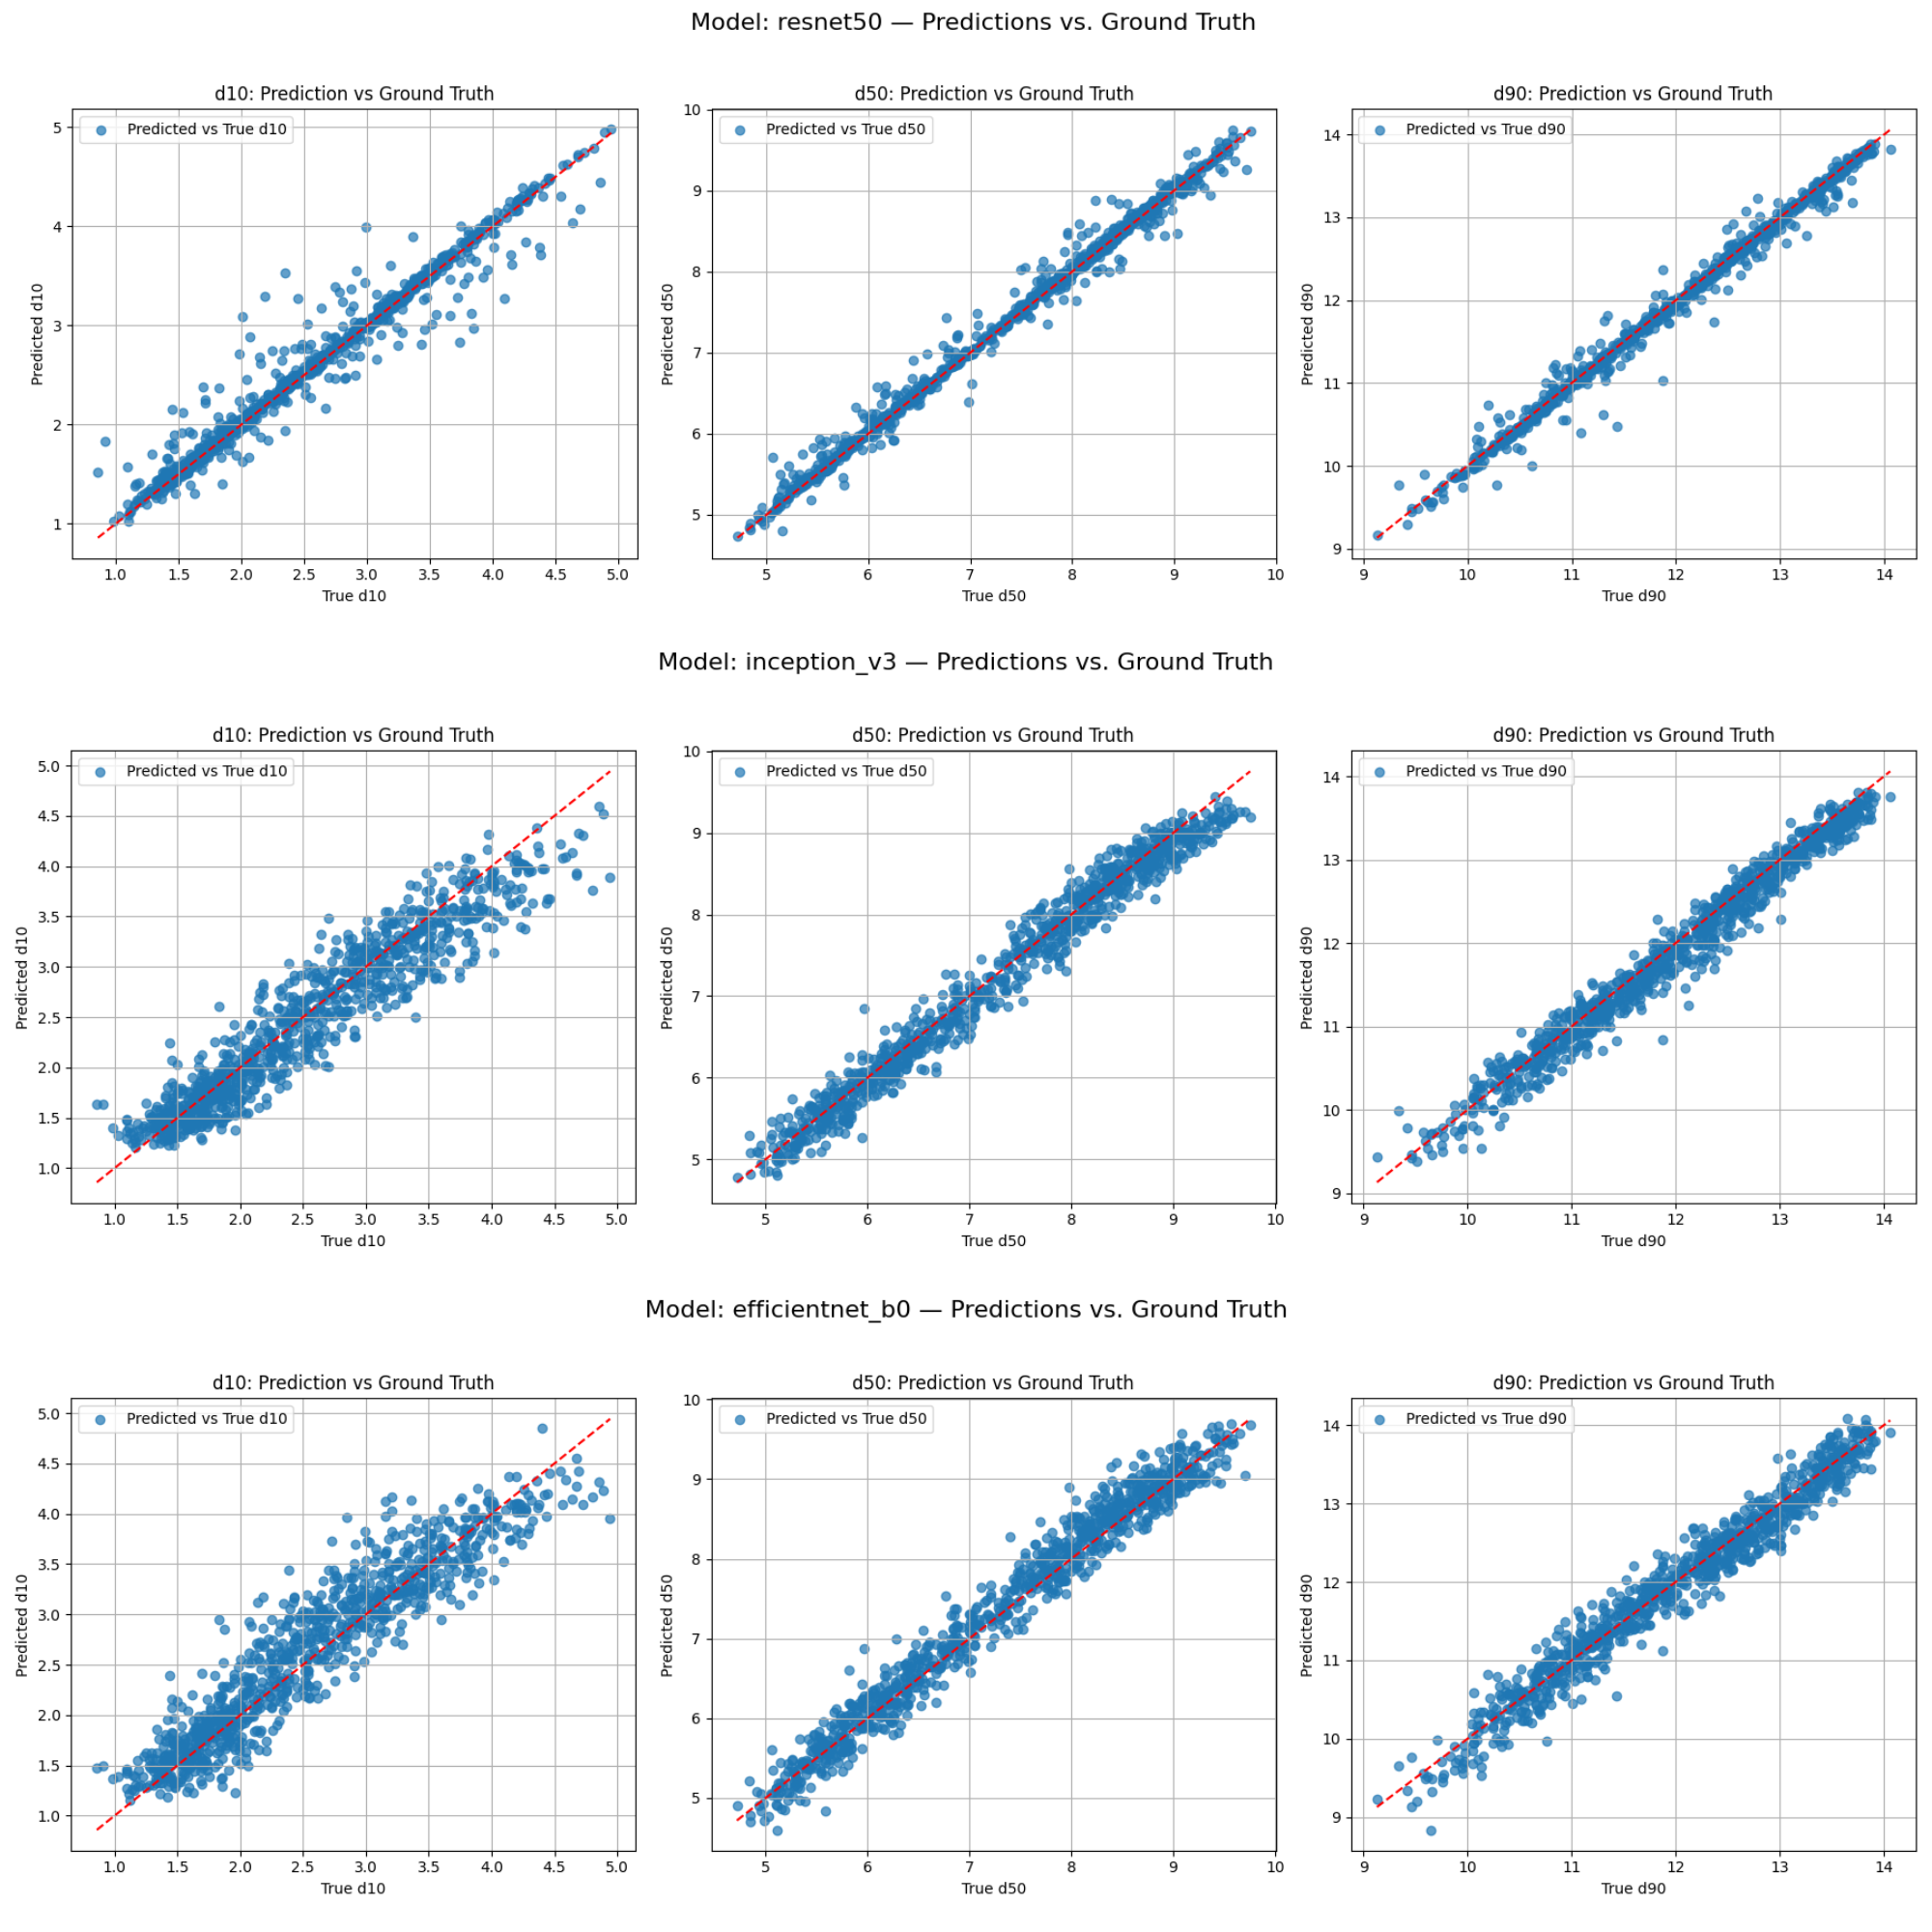
\includegraphics[width=1\textwidth]{Synthetic_Data_for_Computer_Vision___CVPR_2025/figures/true_vs_pred.png}
        \caption{Predicted vs. ground truth PSD values on synthetic test data for all three CNN models.}
        \label{fig:pred-vs-truth}
  \end{figure}

  \heading{Computational Efficiency}
  
  EfficientNet-B0 offers best speed/accuracy trade-off: 37.75 FPS (GPU) vs. ResNet-50's 27.31 FPS, with 5× fewer parameters (5.3M vs. 25.6M), making it ideal for real-time industrial deployment on commodity hardware.

  \begin{table}[htbp]
  \centering
  \caption{Model performance and efficiency comparison on laptop hardware (RTX 3060 GPU, AMD Ryzen 7 5800H CPU).}
  \label{tab:efficiency}
  \small
  \begin{tabular}{@{\hspace{0.5em}}l@{\hspace{0.8em}}c@{\hspace{0.8em}}c@{\hspace{0.8em}}c@{\hspace{0.8em}}c@{\hspace{0.8em}}c@{\hspace{0.5em}}}
  \hline
  \rule{0pt}{2.5ex}\textbf{CNN Model} & \textbf{R² Score} & \textbf{GPU FPS} & \textbf{CPU FPS} & \textbf{Time/Img (s)} & \textbf{Params (M)} \\[0.5ex]
  \hline
  \rule{0pt}{2.5ex}ResNet-50          & \textbf{0.9987}   & 27.31   & 14.66   & 0.0366             & 25.6            \\[0.5ex]
  InceptionV3        & 0.9966   & 23.18   & 12.00   & 0.0431             & 23.9            \\[0.5ex]
  EfficientNet-B0    & 0.9959   & \textbf{37.75}   & \textbf{21.51}   & \textbf{0.0265}  & \textbf{5.3}   \\[0.5ex]
  \hline
  \end{tabular}
  \end{table}

  \end{block}

  \begin{block}{Conclusion \& Future Work}
  
  \textbf{Our Contribution:} We present an open-source, fully automated Blender-based pipeline for generating realistic synthetic particle datasets with perfect PSD labels (d10, d50, d90). This eliminates costly manual annotation while enabling robust CNN training for real-time industrial PSD measurement.
  
  \textbf{Results:} ResNet-50 achieves highest accuracy (R²=0.9987), while EfficientNet-B0 delivers optimal speed/accuracy balance (38 FPS, 5.3M params) for deployment. This work was accepted and published at the \textit{Synthetic Data for Computer Vision Workshop, CVPR 2025, Nashville, TN}.
  
  \textbf{Future Work:} Domain adaptation with incremental fine-tuning on limited real data to bridge the synthetic-to-real gap, and edge device deployment for decentralized industrial monitoring.

  \end{block}

  \begin{block}{Open-Source Resources}
  
  The paper and the code for data generation and training are made public. You can access them by scanning the QR codes below.
  
  \vspace{0.5em}
  
  \begin{minipage}[t]{0.48\textwidth}
    \centering
    
\includegraphics[width=0.6\linewidth]{qr_paper.png}
    
    \textbf{SynData4CV CVPR Paper}
  \end{minipage}\hfill
  \begin{minipage}[t]{0.48\textwidth}
    \centering
    
\includegraphics[width=0.6\linewidth]{qr_github.png}
    
    \textbf{Source Code}
  \end{minipage}

  \end{block}

\end{column}
\separatorcolumn



\end{columns}
\end{frame}

\end{document}
